\documentclass[10pt,a4paper]{report}
%\usepackage[left=1cm,right=1cm,top=1cm,bottom=1cm,bindingoffset=0cm]{geometry}
\usepackage[T2A]{fontenc}
\usepackage[utf8]{inputenc}
\usepackage[russian]{babel}
\usepackage{cmap}
\usepackage{amsmath}
\usepackage{amsfonts}
\usepackage{amssymb} 
\usepackage{hyperref}
\usepackage{stackrel}
\usepackage{graphicx}
%\widetilde
\nonfrenchspacing
\righthyphenmin=2
\def\jo{\"e}
\def\num{\textnumero}

%%%%% Формулы
\def\le{\leqslant} % Делает знак неравенства классическим
\def\ge{\geqslant}
\def\emptyset{\varnothing} % Обычное пустое множество
\def\divisible#1#2{#1\hspace{2.5pt}\raisebox{-1.5pt}{\smash{\vdots}}\hspace{2.5pt}#2}
\def\eqmod#1#2#3{#1\equiv#2\mbox{\hspace{2mm}(mod $#3$)}}
\def\so{\Rightarrow}
\def\theoremend{\hfill\vbox to 0pt{\hbox{$\square$}}}
\def\solutionend{\hfill$\blacksquare$}
\def\quest#1{\stackrel{?}{#1}}
\def\epsilon{\varepsilon}
\def\phi{\varphi}
\def\rddots#1{\cdot^{\cdot^{\cdot^{#1}}}} % Зеркальное отражение \ddots
%\def\modop{\ \ \mbox{mod}\ \ }

\def\missing{\rule[-0.33em]{1em}{1.36em}\fbox{???}\rule[-0.33em]{1em}{1.36em}}
\def\missingwhat#1{\fbox{\parbox{10cm}{#1}}}


\def\df{{\bfseries Определение. }}
\def\pr#1{{\bf Задача \num#1. }}
\def\th{{\bfseries Теорема. }}
\def\bigmid{\mathrel{}\middle|\mathrel{}}
\def\solutionstart{$\square$\;\;}
\def\therm#1{{\it #1}}

\usepackage{indentfirst}
\DeclareMathOperator{\Mat}{Mat}
\DeclareMathOperator{\M}{M}
\DeclareMathOperator{\Sp}{Sp}
\DeclareMathOperator{\Tr}{Tr}
\DeclareMathOperator{\tr}{tr}
\DeclareMathOperator{\Def}{def}
\DeclareMathOperator{\id}{id}
\DeclareMathOperator{\odd}{odd}
\DeclareMathOperator{\Det}{Det}
\DeclareMathOperator{\Vol}{Vol}
\DeclareMathOperator{\sign}{sign}
\DeclareMathOperator{\sgn}{sgn}
\DeclareMathOperator{\Id}{Id}
\DeclareMathOperator{\ord}{ord}
\DeclareMathOperator{\adj}{adj}
\DeclareMathOperator{\rk}{rk}
\DeclareMathOperator{\re}{Re}
\DeclareMathOperator{\Ker}{Ker}
\DeclareMathOperator{\im}{Im}
\DeclareMathOperator{\Arg}{Arg}
%\DeclareMathOperator{\ch}{ch}
%\DeclareMathOperator{\ker}{ker}
\DeclareMathOperator{\Rg}{Rg}
\DeclareMathOperator{\Dom}{Dom}
\DeclareMathOperator{\diag}{diag}
\DeclareMathOperator{\Gr}{Gr}
\DeclareMathOperator{\Tor}{Tor}
\DeclareMathOperator{\ort}{ort}
\DeclareMathOperator{\PR}{pr}
\DeclareMathOperator{\grad}{grad}
\DeclareMathOperator{\rank}{rank}
\DeclareMathOperator{\Char}{char}
\DeclareMathOperator{\Int}{int}
\DeclareMathOperator{\Ext}{ext}
\DeclareMathOperator{\diam}{diam}
\DeclareMathOperator{\cov}{cov}
\DeclareMathOperator{\dom}{dom}

\def\deflr{\stackrel[\Def]{}{\Longleftrightarrow}}

\def\dvec#1#2{\begin{pmatrix}
#1\\#2
\end{pmatrix}}
\def\ov#1{\overrightarrow{#1}}
\def\ovl#1{\overline{#1}}
\def\mat#1#2#3{\begin{pmatrix}
#1_{11} & #1_{12} & \ldots & #1_{1#3}\\
\vdots &  & \ddots & \vdots \\
#1_{#2 1} & #1_{#2 2} & \ldots & #1_{#2#3}
\end{pmatrix}
}
\def\vec#1#2{\left(\begin{smallmatrix}#1\\\vdots\\
#2\end{smallmatrix}\right)}
\def\system#1#2{\left\{
\begin{aligned}
#1\\
\vdots\\
#2\\
\end{aligned}
\right.
}
\def\blockmatrix#1#2#3#4{\left(
\begin{array}{c|c}
  #1 & #2 \\ \hline
  #3 & #4
\end{array}
\right)}


\def\Uc{\stackrel{\circ}{U}}
\def\rra#1{\stackrel{#1}{\rightrightarrows}}
\def\E{\mathbb E}
\def\D{D}
\def\vrt#1{\left\lVert#1\right\rVert}
\def\br#1{\left(#1\right)}
\def\brc#1{\left\{#1\right\}}
\def\abs#1{\left|#1\right|}
% \stackrel stackbin 

\usepackage{setspace}
\begin{document}
\setstretch{1.4}

\chapter{Алгоритмы визуализации данных на клиенте}

В данной главе описываются реализации двух алгоритмов визуализации данных: Fruchterman Reingold и t-SNE.

Несмотря на наличие множества реализаций этих алгоритмов на JavaScript, ни одна из них не использует GPU. При этом нет простого способа портировать существующие реализации этих алгоритмов на GPU с других языков программирования, так как WebGL API очень ограничен по сравнению с OpenGL и другими API для графических карт.

\section{WebGL для обработки данных}
\label{sec:webgl_data_analysis}

Операция \texttt{break} будет работать корректно, однако затраченное время будет пропорционально верхней оценке, то есть остальные итерации будут выполнены вхолостую.

Продвинутые графические карты способны определять момент, когда все циклы были остановлены, чтобы уменьшить время выполнения. Тем не менее, было бы некорректно предполагать наличие этой функциональности у всех пользователей при рассчете сложности алгоритма.

\section{Fruchterman Reingold}

Это классический алгоритм рисования графа из категории force-directed drawing.

Он использует физическую аналогию, в которой ребрам соответствуют пружины, а вершинам --- одинаково заряженные частицы. Таким образом, соединенные ребром вершины стремятся быть на фиксированном расстоянии друг от друга, равном оптимальной длине пружины, а не соединенные вершины отталкиваются друг от друга.

На практике, закон Гука для силы пружины не используется, так как он слишком сильно действует на соединенные вершины, находящиеся в разных частях графа.

Для алгоритма Fruchterman Reingold силы притяжения и отталкивания равны $f_a(d) = d^2 / k$ и $f_r(d) = -k^2 / d$, где $k$ --- оптимальная длина пружины, при которой эти силы сбалансированы.

Обычно, физическая симуляция осуществляется при помощи интегрирования Верле, но в этом алгоритме силы по сути являются скоростями, так как это ускоряет сходимость.

Алгоритм начинает со случайных позиций вершин и останавливается, когда система достигает равновесия. Для ускорения этого процесса вводится понятие {\itshape температуры}, которая ограничивает максимальное изменение положения вершин и уменьшается по заданному закону.

\section{t-SNE}

Применение этого алгоритма считается одним из наиболее мощных методов уменьшения размерности до 1-3 измерений.

В базовой версии он получает на вход множество точек $\brc{x_i}$ в пространстве большой размерности (например, 50), а также начальное случайное положение представлений этих точек $\brc{y_i}$ в пространстве размерности 1-3. Для точек $x_i$ предрассчитывается матрица расстояний $\br{p_{ij}}$ по формуле:

$$p_{ij} = \frac{p_{i|j} + p_{j|i}}{2}$$

$$p_{j|i} = \frac{\exp(-\vrt{x_i - x_j}^2 / 2 \sigma_i^2)}{\sum_{k\neq i}\exp(-\vrt{x_i - x_k}^2 / 2 \sigma_i^2)},$$
где $\sigma_i$ подбираются при помощи двоичного поиска так, чтобы для всех $i$:
$$-\sum_j p_{j|i} \log_2 p_{j|i} = \log_2(\mbox{\itshape perplexity}),$$
где {\itshape perplexity} является параметром алгоритма.

Описанные выше вычисления производятся один раз при инициализации алгоритма. Далее происходят итерации, на каждой из которых вычисляется матрица $\br{q_{ij}}$:

$$ q_{ij} = \frac{(1 + \vrt{y_i - y_j}^2)^{-1}}{\sum_{k\neq l}(1 + \vrt{y_k - y_l}^2)^{-1}},$$
после чего для каждой вершины $y_i$ считается градиент целевой функции:

$$\Delta y_i = 4 \sum_j (p_{ij} - q_{ij}) (y_i - y_j),$$
на основании чего считаются новые положения $y_i$ и итерация повторияется. При вычислении новых положений предлагается использовать {\itshape momentum term}:
$$y_i^{t} = y_i^{t - 1} + \eta \Delta y_i + \alpha(t)(y_i^{t - 1} - y_i^{t - 2}),$$
где $\eta$ --- фиксированная константа, $\alpha(t)$ --- убывающая функция, $y_i^t$ --- значение $y_i$ после итерации $t$.

\section{Схема вычислений.}

Два приведенных алгоритма имеют общую структуру:

\begin{verbatim}
const edges: buffer[m] = serialize_edges()
positions: buffer[n, dim] = random_positions()
attractions, repulsions: buffer[n, dim]
grid: structure
finished: boolean = false
iteration: integer = 0

while not finished:
    iteration += 1
    attractions = calc_attractions(positions, edges)
    grid = calc_grid(positions)
    repulsions, norm_sum = calc_repulsions(positions, grid)
    positions, finished = calc_positions(
        positions,
        attractions,
        repulsions,
        iteration,
        norm_sum,
    )
\end{verbatim}

Здесь \texttt{n} --- число вершин, \texttt{m} --- число ребер, \texttt{dim} --- размерность пространства визуализации (от 1 до 3).

На вход алгоритму поступают два буффера: \texttt{edges} и \texttt{positions}. Позиции инициализируются случайными числами в заданных пределах. Ребра преобразуются в буффер при помощи одной из нескольких схем, перечисленных далее.

После этого следует некоторое число итераций. Для алгоритма Fruchterman Reingold номер итерации нужен для уменьшения температуры со временем, t-SNE останавливается, когда вершины пересают менять положение больше, чем на $\varepsilon$.

Силы притяжения действуют только между парами вершин, соединенных ребром. Таким образом, вычисление сумм этих сил для всех вершин не возможно без прохода по всем ребрам, т.е. за $O(m)$ времени и памяти. Улучшение скорости этой части возможно через уменьшение числа ребер.

Силы отталкивания действуют между всеми парами вершин, что позволяет делать некоторые оптимизации, при этом уменьшая точность этих вычислений на несколько процентов. Сложность этой части варьируется $O(n\log n)$ до $O(n^2)$ по времени и $O(n)$ по памяти.

Для алгоритма t-SNE требуется вычисление нормирующего множителя, равному сумме всех ненормированных сил притяжения между всеми парами вершин. 

При использовании оптимизаций требуется дополнительная структура \texttt{grid}, которая требует одного прохода по позициям вершин и $O(n)$ памяти.

Последняя функция \texttt{calc\_positions} также проходит по всем вершинам, при этом она может содержать дополнительную логику, которая проверяет, нпример, выход вершин за границы ограничивающего прямоугольника.

Исходя из приведенных выше оценок, лучше всего для исполнения на GPU подходят функции \texttt{calc\_attractions} и \texttt{calc\_repulsions}.

\section{Выбор ребер и их представление}

Вычисление сил притягивания определяется выбором подмножества ребер и способом их представления в виде текстуры.

Рассмотрим три способа выбора ребер:
\begin{itemize}
\item[(a)] Все ребра.
\item[(b)] Оставить не более $k$ ребер наибольшего веса у каждой вершины.
\item[(c)] Оставить не более $k$ ребер наибольшего веса у всего графа.
\end{itemize}

Также предлагается четыре способа представления ребер:
\begin{itemize}
\item[(p)] Матрица смежности. Элементы --- веса ребер.
\item[(q)] Матрица $n\times 2k$, в которой строки соответствуют вершинам, в каждой строке слева направо указан список ребер в виде чередующегося списка номеров вершин и весов ребер. $k$ --- наибольшая степень вершины.
\item[(r)] Вектор длины $n + 2m$. Первые $n$ чисел --- <<указатели>> на индексы вектора, с которых начинается список ребер соответствующей вершины. Следующие $2m$ чисел являются объединением списков ребер, выходящих из каждой вершины.
\item[(s)] Матрица $n'\times (1 + 2s)$. Строки соответствуют вершинам, при этом одной вершине может соответствовать несколько подряд идущих строк. Номер вершины, соответствующей данной строке указан в первом столбце. В остальных столбцах указан список ребер и их весов. Если степень вершины больше $s$, она занимает несколько строк.
\end{itemize}

Способ (q) лучше всего подходит вместе со способом выбора ребер (b), иначе, если есть хотя бы одна вершина степени $n-1$, то этот способ будет хуже по времени и памяти, чем (p).

Способ (r) требует меньше всего памяти, но, в связи с особенностью работы GPU, время обработки всех вершин будет пропорционально максимальному времени обработки одной вершины, то есть максимальной степени $k$. Если есть хотя бы одна вершина степени $n - 1$, то его время работы будет дольше, чем у способа (p).

Наконец, способ (s) требует не сильно больше памяти по сравнению с (r), при этом наиболее эффективно распараллеливается на GPU. Единственный недостаток состоит в том, что после его применения необходимо аггрегировать результаты строк, соответствующих одной вершине.

\section{Реализация вычисления сил притяжения}
\label{sec:attractions_implementation}

В данном разделе приводится псевдокод реализации функции \texttt{calc\_attractions} для представления ребер (s). Его несложно упростить для представления (q).

Для хранения информации о ребрах используется RGBA-текстуры вместо floating point. Это позволяет хранить два 16-битных числа в одном пикселе. Первое число используется для номера вершины в списке ребер (которых будет значительно меньше 65536), а второе --- для веса ребра. Такое представление уменьшит точность хранения весов ребер, но, с учетом того, что веса ребер входят в формулы линейно и не связаны уравнениями с другими переменными, это не должно значительно ухудшить качество визуализации.

Значение 0 для веса ребер означает отсутствие ребра. Это может потребоваться, чтобы заполнить оставшиеся ячейки в строках представления (s). Первая колонка матрицы, кодирующая номер вершины, соответствующей данной строке, использует только первое 16-битное число.

Результатом работы шейдера будут являться $dim$ вещественных текстур $1\times n$, содержащих вектора сил, действующих на вершины от ребер по строкам.

На вход шейдер получает текстуру \texttt{edges} размера $n'\times(1 + s)$ и текстуру \texttt{positions} размера $n\times dim$. Для каждой размерности \texttt{dim} код компилируется отдельно.

Псевдокод шейдера для $dim = 2$:

\begin{verbatim}
const S: integer;
const MAX_WEIGHT: float;

int high(rgba pixel): pixel.r * 256 + pixel.g
int low(rgba pixel): pixel.b * 256 + pixel.a

calc_attractions(chunk_no):
    int source = high(edges[chunk_no, 0])
    float x = positions[source, 0]
    float y = positions[source, 1]
    float x_sum = 0, y_sum = 0
    for i = 1 ... S:
        rgba edge_pixel = edges[chunk_no, i]
        float weight = low(edge_pixel) / 256 / 256 * MAX_WEIGHT
        if weight == 0: break
        int target = high(edge_pixel)
        float dx = positions[target, 0] - x
        float dy = positions[target, 1] - y
        float sq_dist = dx ^ 2 + dy ^ 2
        float mul = calc_attr_mul(sq_dist, weight)
        x_sum += mul * dx, y_sum += mul * dy
    return x_sum, y_sum
\end{verbatim}

Функция \texttt{calc\_attr\_mul} зависит от реализуемого алгоритма:

\begin{verbatim}
calc_attr_mul_fuchterman_reingold(float sq_dist, float weight):
    return weight * sq_dist / K

calc_attr_mul_tsne(float sq_dist, float weight):
    return weight / (sq_dist + 1)
\end{verbatim}

\section{Подходы к оптимизации вычисления сил отталкивания}

% https://habr.com/post/341208/

В обоих алгоритмах <<узким местом>> по времени выполнения является вычисление сил отталкивания между всеми парами вершин. В данной работе рассматриваются три подхода к этому:

\begin{itemize}
\item[(k)] Вычислять отталкивание между всеми парами вершин.
\item[(l)] Вычислять отталкивание только между близкими вершинами.
\item[(m)] Группировать вершины при вычислении отталкивания на большом расстоянии.
\end{itemize}

Подход (l) рекомендуется создателями Fruchterman Reingold, подход (m) испоьзуется во многих реализациях подобных алгоритмов визуализации данных.

В связи с ограничениями шейдеров WebGL, в данной работе в методе (m) может вычисляться только силы между двумя вершинами или между вершиной и группой вершин, а не между двумя группами вершин.

Чтобы применить оптимизации (l) и (m), необходимо иметь дополнительную структуру, позволяющую получать группы близких вершин, желательно на разных масштабах.

Существует множество подобных структур, мы рассмотрим только две из них:

\begin{itemize}
\item[(x)] Прямоугольная 1,2,3-мерная сетка.
\item[(y)] Двоичное/квадро-/окто-дерево.
\end{itemize}

Сочетание (m)(y) называется Barnes-Hut simulation.

\section{Представление иерархии клеток в виде текстуры}

\label{sec:struct_texture}

Предлагаемый способ обладает следущими характеристиками:

\begin{itemize}
\item Вычисление на CPU за линейное от числа вершин время и потребление памяти.
\item Поддержка как прямогольних сеток, так и различных древовидных иерархий клеток.
\item Клетки могут иметь любую форму.
\item Поддержка 1, 2 и 3 измерений.
\item Возможность пропуска дочерних клеток, в которых нет вершин.
\item Возможность получить список вершин для клеток любого уровня.
\item Центр клетки может совпадать с центром ограничивающего прямоугольника (отрезка, параллелепипеда), либо может совпадать с центром масс входящих в него точек.
\item Прямоугольный массив клеток одного уровня можно обойти за линейное время (без необходимости повторять бинарный поиск для каждой клетки).
\end{itemize}

Также для этой иерархии требуется дополнительная текстура, содержащая отсортированный список номеров вершин. Номера должны быть отсортированы так, чтобы множество номеров внутри клетки любого уровня шло подряд в отсортированном списке. Это можно получить при помощи обхода дерева.

В основной текстуре строки взаимно однозначно соответствуют клеткам. При этом строки отсортированы по такому же принципу, что и дополнительная структура, т.е. все потомки любой клетки должны идти подряд в основной текстуре сразу после строки, соответствующей родительской клетке. Эти свойства выполняются при обходе дерева.

Как основная, так и дополнительная текстуры имеют формат RGBA и каждый пиксель используется как пара 16-битных целых чисел (для упрощения обработки, дополнительная текстура использует только первые числа пар). Эти два числа будут обозначаться суффиксами L и H.

Для указания координат и размеров используются 16-битные числа. Это не должно значительно повлиять на качество работы алгоритма т.к. такими числами кодируются лишь центры и размеры клеток, а координаты вершин и их силы по-прежнему представлены 32-битными вещественными числами. Если клетки делятся степенями двоек, как в Barnes-Hut, то 16-битные числа будут точно приближать центры клеток (но не радиусы, т.к. они будет домножаться на $\sqrt{2}$).

Вместе с текстурой должна передаваться константа, отражающая масштабный коэффициент для 16-битных чисел. Ее рекомендуется подбирать так, чтобы значение 65535 соответствовало максимуму из ширины и высоты ограничивающего прямоугольника.

В основной текстуре столбцы устроены следующим образом:

\begin{itemize}
\item[0H] Размер клетки --- сторона квадрата с центром в центре клетки, целиком содержащего все вершины клетки.
\item[0L] Номер следущего потомка такого же уровня в дереве. Если текущая клетка является последним потомком, то номер следующей клетки после родительской и т.д. Если это самая последняя клетка, то записать 0.
\item[1, 2] Координаты центра клетки ($x\to 1H, y\to 1L, z\to 2H$) и количество вершин в ней (2L). В случае менее трех измерений неиспользуемые координаты равны нулю.
\item[3H] Индекс первой вершины данной клетки в дополнительной текстуре.
\item[3L] Индекс последней вершины данной клетки в дополнительной текстуре.
\item[4H] Номер клетки справа от текущей или 0, если такой нет. Эта клетка может не быть смежной с текущей в случае, если правая смежная клетка была пропущена.
\item[4L] Номер клетки под текущей или 0, если такой нет. Аналогично, эта клетка не обязательно должна быть смежной.
\item[5H] Номер клетки за текущей для трехмерного случая или 0.
\end{itemize}

\section{Особенности реализации иерархии клеток}
\label{sec:cells_implementation}

Структура, описанная в предыдущем разделе, довольно общая и для одного набора позиций вершин допускает множество построений с разными формами клеток и глубиной их вложенности. Также в связи с особенностями работы графической карты (описанные в разделе \ref{sec:iter_estimate}) для этой структуры должна быть возможность получить оценки на время обхода вершин и клеток.

Клетки структуры будут квадратными, центр клеток совпадает с центром квадрата. Центр масс вершин клетки в качестве центра клетки не используется, так как для этого необходимо считать радиус и центр описанной окружности входящих в квадрат вершин, что может потребовать больше времени CPU, при том, что время GPU останется прежним, это лишь отразится на точности.

Потребуем, чтобы при перечислении потомков клетки их порядок согласовался с направлениями, используемыми в столбцах 4H, 4L и 5H. То есть слева-направо, сверху-вниз, от передних клеток к задним.

При построении иерархии главными параметрами будут максимальная допустимая погрешность вычисления расстояния $\lambda$, а также максимальный уровень $l$ (нумерация начинается с нуля).

Для упрощения рассчетов, будем считать, что ограничивающая область является квадратом со стороной 1. Если область прямоугольная, то в функции \texttt{calc\_positions} необходимо откорректировать логику проверки выхода за границы.

Получаем, что для клетки уровня $i$ сторона квадрата равна $2^{-i}$, максимальное расстояние от вершины до центра клетки не больше $2^{-i} / \sqrt{2}$. Таким образом, при рассчете расстояния от некоторой точки до группы вершин клетки, в случае замены группы на центр клетки, погрешность не будет превосходить $2^{-i - 0.5} / x$.

Посчитаем радиус $r_0$, на котором квадрат последнего уровня не может приближать расстояние с приемлимой точностью, то есть на котором необходимо обрабатывать вершины по одной:  $2^{-l - 0.5} / x \ge \lambda$, то есть $r_0 = 2^{-l - 0.5} / \lambda$.

Посчитаем наименьший уровень $l_0$, который может обеспечить приемлимое приближение в пределах ограничивающего квадрата. Наибольшее расстояние между вершиной и клеткой в нем не больше $\sqrt{2}$, тогда $2^{-l_0 - 0.5} / \sqrt{2} \le \lambda$, следовательно $l_0 =  \log_2(1 / \lambda) - 1$.

\section{Локальные и глобальные силы отталкивания}
\label{sec:iter_estimate}

\begin{figure}[h!]
  \centering
  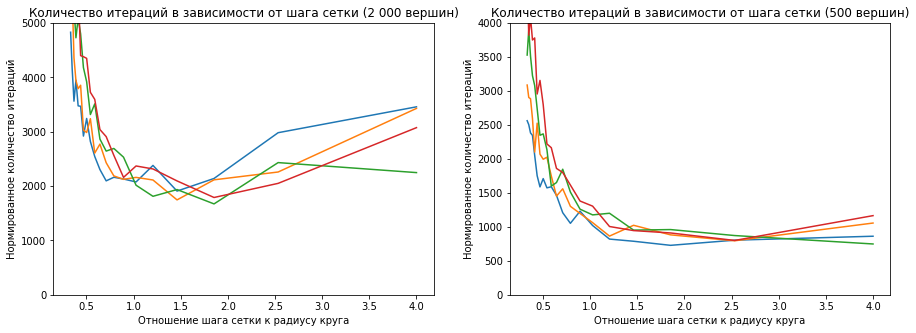
\includegraphics[width=\textwidth]{grid_step_2.png}
  \caption{Моделирование числа итераций локальных сил отталкивания для разных шагов сетки, значений $r_0$ и количеств вершин для размерности 2.}
  \label{fig:grid_step}
\end{figure}

Из-за неэффективой обработки условий в шейдерах WebGL, вычисление сил отталкивания будет проходить в два цикла: для {\bfseries локальных сил отталкивания} (для которых требуется обрабатывать вершины по одной) и {\bfseries глобальных} (когда считается силы между вершиной и клеткой).

При вычислении локальных сил, необходимо итерироваться по вершинам, входящих в некоторые клетки. Это добавляет еще один вложенный цикл, количество итераций которого равно максимальному числу вершин во всех клетках.

Таким образом имеется три цикла, для которых необходимо иметь верхнюю оценку на число итераций (см. главу \ref{sec:webgl_data_analysis}). Оставшаяся часть этой главы будет посвящена объяснению выбора такой константы для последнего (вложенного) цикла, так как это влияет на реализацию алгоритма. Оценки для первых двух циклов будут даны в главе \ref{sec:repulsion_time} после главы с псевдокодом шейдера.

С учетом того, что число итераций вложенного цикла должно быть постоянным, имеет смысл брать лишь клетки одного уровня, так как в клетках разных уровней в разы отличается число входящих в них вершин.

Тогда задача состоит в том, чтобы найти шаг сетки, относительно круга радиуса $r_0$, для которых суммарное количество итераций наименьшее. Итерации происходят следующим образом. Выбираются те клетки, описанная окружность которых пересекаются с кругом радиуса $r_0$. Затем происходит обход вершин в выбранных клетках за время, равное произведению максимума числа вершин в во всех клетках сетки на число выбранных клеток.

При малом шаге сетки, у количества вершин в клетках будет большая дисперсия, а, следовательно, и максимум. При этом суммарная площадь выбранных клеток будет не сильно отличаться от площади круга. При большом шаге сетки, максимум количества вершин будет не значительно отличаться от среднего количества, но суммарная площадь выбранных клеток будет в разы больше площади круга.

Также следует заметить, что количество выбранных клеток зависит от положения центра круга относительно сетки и является случайной величиной. Но в реализации алгоритма число итераций должно равняться верхней оценке этого числа.

На рисунке \ref{fig:grid_step} показаны результаты моделирования количества итераций по схеме, описанной выше. Два графика показывают результаты при разном количестве вершин от $2\ 000$ и $500$. Разные линии в одном графике получены при разных значениях радиуса $r_0 = 1 / 20 \ldots 1 / 50$. Это соответствует разбросу параметров, например, от $7.5\%$ до $20\%$ точности при 8 уровнях. Наконец, каждая точка каждой линии была получена усреднением результатов на 10 случайных конфигурациях вершин. Вершины были равномерно распределены по квадрату. Так как при разных радиусах количество итераций значительно отличается, значения для каждой линии были домножены на величину, обратную радиусу, чтобы их можно было нанести на один график.

Как оказалось, оптимальный шаг сетки отличается при разной плотности вершин, но, в целом оптимальное значение находится в пределах $1.0 r_0 \ldots 2.0 r_0$. Для трех измерений шаг был около $2r_0\ldots 5r_0$.

В данной работе заначение шага сетки полагается равным $2r_0$. Помимо того, что оно находится в пределах оптимальных значений, для него количество клеток, которые пересекает круг, не превосходит 4, при этом эти четыре клетки содержатся в квадрате $2\times 2$, клетки которого можно получить при помощи столбцов 4H и 4L.

Так как клетки имеют стороны, равные обратным степеням двойки, шаг сетки выбирается как ближайшая сверху обратная степень двойки. Этот шаг хранится в константе \texttt{LOCAL\_GRID\_SIZE}.

Для того, чтобы иметь возможность итерироваться по клеткам квадрата $2\times 2$ в построенной выше сетки, необходимо потребовать, чтобы при построении дерева все клетки размера \texttt{LOCAL\_GRID\_SIZE} присутствовали, даже если в них нет вершин. Это увеличит размер текстуры для клеток, но ускорит процесс их прохода на GPU.

\section{Вычисление сил отталкивания при помощи иерархии клеток}

Структура для оптимизации вычисления сил отталкивания называется \texttt{grid} и имеет следующий поля:

\begin{itemize}
\item \texttt{grid.cells} --- RGBA текстура $4\times s$, где $s$ --- количество клеток.
\item \texttt{grid.vertices} --- дополнительная RGBA текстура, содержащая отсортированные номера вершин (см. описание в разделе \ref{sec:struct_texture}).
\item \texttt{grid.scale} --- вещественная константа, на которую домножаются 16-битные длины и координаты.
\end{itemize}

Далее приведен псевдокод шейдера вычисления сил отталкивания для размерности 2. Функции \texttt{low} и \texttt{high} приведены в листинге главы \ref{sec:attractions_implementation}.

\begin{verbatim}
calc_repulsions(vertex_no):
    float x = positions[vertex_no, 0]
    float y = positions[vertex_no, 1]
    float s = grid.scale
    int cell_no = 0
    float x_sum = 0, y_sum = 0, norm_sum = 0
    int top_left_cell_no = CELLS_COUNT

    for i = 1 .. GLOBAL_MAX_ITER:
        float side = high(grid.cells[cell_no, 0]) * s
        float dx = high(grid.cells[cell_no, 1]) * s - x
        float dy = low(grid.cells[cell_no, 1]) * s - y
        float sq_dist = dx ^ 2 + dy ^ 2
        float sq_accuracy = side ^ 2 / 2 / sq_dist;
        int next = low(grid.cells[cell_no, 0])
        int chebyshev = max(abs(dx), abs(dy))
        if grid_size == LOCAL_GRID_SIZE
           and chebyshev < side + LOCAL_GRID_SIZE:
             top_left_cell_no = min(top_left_cell_no, cell_no)
             cell_no = next
        elif sq_accuracy < SQ_MAX_ACCURACY:
            int count = low(grid.cells[cell_no, 2])
            float mul = calc_rep_mul(sq_dist) * mul
            norm_sum += mul
            x_sum += mul * dx, y_sum += mul * dy
            cell_no = next
        else:
            cell_no += 1
       if cell_no == 0 or cell_no >= CELLS_COUNT: break

    top_right_cell_no = high(grid.cells[top_left_cell_no, 4])
    bottom_left_cell_no = low(grid.cells[top_left_cell_no, 4])
    bottom_right_cell_no = high(grid.cells[bottom_left_cell_no, 4])

    x_add, y_add, norm_add = calc_local_forces(x, y, top_left_cell_no)
    x_sum += x_add, y_sum += y_add, norm_sum += norm_add
    x_add, y_add = calc_local_forces(x, y, top_right_cell_no)
    x_sum += x_add, y_sum += y_add, norm_sum += norm_add
    x_add, y_add = calc_local_forces(x, y, bottom_left_cell_no)
    x_sum += x_add, y_sum += y_add, norm_sum += norm_add
    x_add, y_add = calc_local_forces(x, y, bottom_right_cell_no)
    x_sum += x_add, y_sum += y_add, norm_sum += norm_add

    return x_sum, y_sum

calc_local_forces(x, y, cell_no)
    int vertex_min_idx = high(grid.cells[cell_no, 3])
    int vertex_max_idx = low(grid.cells[cell_no, 3])
    int cur_vertex_idx = vertex_min
    float x_sum = 0, y_sum = 0, norm_sum = 0
    for i = 1 .. MAX_GRID_VERTICES:
        if cur_vertex_idx > vertex_max_idx: break
        int vertex_no = low(grid.vertices[cur_vertex_idx])
        float dx = positions[vertex_no, 0] - x
        float dy = positions[vertex_no, 1] - y
        float sq_dist = dx ^ 2 + dy ^ 2
        float mul = calc_rep_mul(sq_dist)
        x_sum += dx * mul, y_sum += dy * mul, norm_sum += mul
        cur_vertex_idx += 1
    return x_sum, y_sum, norm_sum
\end{verbatim}

При вычислении локальных сил отталкивания расстояние возводится в квадрат, чтобы не брать квадратный корень.  Для определения пересечения квадратов используется расстояние Чебышева.

\begin{itemize}
\item Константа \texttt{SQ\_MAX\_ACCURACY} равна $\lambda^2$.
\item Константа \texttt{LOCAL\_GRID\_SIZE} равна шагу сетки, вычесленному в предыдущем разделе.
\item Константа \texttt{MAX\_GRID\_VERTICES} содержит максимальное количество вершин в клетке размера шага сетки. Предполагается, что во время выполнения обоих алгоритмов не будет клеток, в которых содержится значительно большее среднего число вершин.
\item Константа  \texttt{CELLS\_COUNT} содержит общее число клеток.
\item Переменная \texttt{top\_left\_cell\_no} хранит номер верхней левой клетки из тех четырех, которые используются для вычисления локальных сил отталкивания.
\item Переменная \texttt{norm\_sum} нужна для подсчета сумм норм в t-SNE, в Fruchterman Reingold её можно удалить.
\end{itemize}

Функция \texttt{calc\_rep\_mul} зависит от алгоритма:
\begin{verbatim}
calc_rep_mul_fruchterman_reingold(sq_dist):
    return -K_SQUARED / sqrt(sq_dist)

calc_rep_mul_tsne(sq_dist):
    return 1 / (1 + sq_dist)
\end{verbatim}

Константа \texttt{K\_SQUARED} равна квадрату \texttt{K} --- оптимальной длинны ребра в Fruchterman Reingold.

\section{Оценка времени вычисления сил отталкивания.}
\label{sec:repulsion_time}

Осталось найти оценку для константы \texttt{GLOBAL\_MAX\_ITER}, равной максимальному числу посещенных клеток при подсчете сил от одной вершины.

Сначала оценим количество вершин в дереве с $l$, $u$ листьями и не более $d$ потомками у каждого родителя. Пусть $l' = \lfloor\log_d u\rfloor$. Тогда первые $l'$ уровней содержат не более
$$d^0 + \cdots + d^{l'} = \frac{d^{l' + 1} - 1}{d - 1} < \frac{d u - 1}{d - 1} < \frac{d}{d - 1}$$
вершин. С другой стороны в каждом уровне число вершин не может превышать число всех листьев, поэтому число вершин в оставшихся $(l - l')$ уровнях не превосходит $u (l - l')$ и всего вершин не более
\begin{equation}
  \br{\frac{d}{d - 1} + l - \lfloor\log_d u\rfloor} u < \br{\frac{d}{d - 1} + l}u = C_1 u
  \label{eq:leafs_count}
\end{equation}

Рассмотрим дерево посещений, состоящее из всех клеток, запрошенных шейдером, приведенном в предыдущем разделе, при обработки одной вершины.

Оценим число листьев в дереве. Рассмотрим клетку со стороной $s$. Её <<радиус>> (то есть максимальное расстояние от вершины до центра квадрата) равен $r = s / \sqrt{2}$. Пусть клетка находятся на расстоянии $x$ от обрабатываемой шейдером вершины. Тогда для погрешности должно выполняться $r / x \le \lambda$. Если клетка является листом, то для её родителя, который в два раза больше, это условие должно нарушаться. Тогда $2r / x' > \lambda$, где $x'$ --- расстояние до центра родителя. Так как центр родителя совпадает с одним из углов дочерней клетки, $x' > x - r$. Получаем
$$\frac{r}{\lambda} \le x < x' + r < \br{\frac{2}{\lambda} + 1} r$$
Тогда все точки всех клеток (явяющихся листьями в дереве посещений) со стороной $s$ находятся в кольце с радиусом:
$$\br{\frac{1}{\lambda} - 1} r \ldots \br{\frac{2}{\lambda} + 2} r$$
Площадь этого кольца равна
$$\pi r^2 \br{(2 / \lambda + 2)^2 - (1/\lambda - 1)^2}$$
Чтобы получить оценку сверху на число квадратов в нем, необходимо разделить его площадь на $s^2 = 2r^2$, в результате получаем оценку
$$u < \frac{\pi}{2}\br{\frac{3}{\lambda^2} + \frac{10}{\lambda} + 3} (l - l_0),$$
где $l_0 = \log_2(1 / \lambda) - 1$ --- верхняя оценка на слой клетки, являющейся листовой (см. главу \ref{sec:cells_implementation}).

Подставляя оценку на $u$ в формулу \ref{eq:leafs_count}, получаем верхнюю оценку на число глобальных итераций.

\section{Результаты испытаний}

\begin{table}[t]
  \centering
  \begin{tabular}{|l l l l l|}
    \hline
     &  & время & $\sigma$ & итераций \\ \hline
    \texttt{attractions} & \texttt{JS} & 0.706 & $\pm 0.023$ & 10 \\ \cline{2-5}
             & \texttt{JS + WebGL} & 0.00111 & $\pm 0.000023$ & 1000 \\\hline
    \texttt{repulsions} & \texttt{C} & 0.671 & $\pm 0.05$ & 10 \\ \cline{2-5}
     & \texttt{asm.js} & 0.514 & $\pm 0.011$ & 10 \\\cline{2-5}
     & \texttt{JS} & 0.504 & $\pm 0.009$ & 10 \\\cline{2-5}
             & \texttt{JS + WebGL} & 0.0247 & $\pm 0.00013$ & 1000 \\\hline
  \end{tabular}
  \caption{Результаты испытаний}
  \label{tab:myfirsttable}
\end{table}

Испытания проводились отдельно для сил отталкивания и притягивания. Измерялось время одной итерации в секундах. Код делился подготовительную и основную часть. В подготовительную часть включалась генерация начальных значений и компиляция. Для реализаций на WebGL время на пересылку от CPU к GPU и обратно включалось в основную часть. Перед началом измерений делалось $30\%$ итераций для <<разогрева>>.

Для сил отталкивания сравнивались простые реализации (имеющие квадратичную сложность) на графе из 4096 вершин. Начальные положения точек генерировались при помощи псевдо-случайного алгоритма с одинаковым начальным значением.

Неожиданный результат был получен при сравнении реализаций на \texttt{C}, \texttt{asm.js} и \texttt{JS}. Код на \texttt{C} был скомпилирован с флагами \texttt{-lm -Ofast}, тем не менее, время его выполнения оказалось на $30\%$ медленнее, чем аналогичного кода на \texttt{JS}, при том, что оптимизированная версия на \texttt{asm.js} показала такой же результат, как и обычная реализация на \texttt{JS}. В реализации на WebGL пересылка от CPU к GPU и обратно проводилась один раз на 10 итераций.

Для сил притягивания использовался граф из 4096 вершин и $4096 \times 1000$ ребер. Каждая вершина имела по 2000 исходящих ребер, константа для схемы (s) равнялась 1000, то есть на каждую вершину приходилось две строки по 1000 ребер. Время вычисления всех сил на GPU (включая пересылку) было сравнимо со временем обхода всех вершин в цикле на JS с выполнением одной простой операции, например, суммы.

\end{document}
